\begin{table}
  \centering
  \caption{Schwingungsdauern bei jeweiligen Abständen.}
  \label{tab:data2}
  \begin{tabular}{c c c c }
    \toprule $a \, \,  in \,\, m$ & $a^2 \,\, in \,\,  m^2$ & $T \,\, in \,\, s$ & $T^2 \,\, in  \,\, s^2$ \\
    \midrule
    0.03 & 0.0009 & 2.06 &  4.2436\\
    0.06 & 0.0036 & 2.29 &  5.2441\\
    0.09 & 0.0081 & 3.21 &  10.3041\\
    0.12 & 0.0144 & 4.16 &  17.3056\\
    0.15 & 0.0225 & 4.81 &  23.1361\\
    0.18 & 0.0324 & 5.41 &  29.2681\\
    0.21 & 0.0441 & 6.38 &  40.7044\\
    0.24 & 0.0579 & 7.16 &  51.2656\\
    0.27 & 0.0729 & 7.52 &  56.5504\\
    0.29 & 0.0841 & 8.49 &  72.0801\\
    \bottomrule
  \end{tabular}
\end{table}

\begin{figure}
  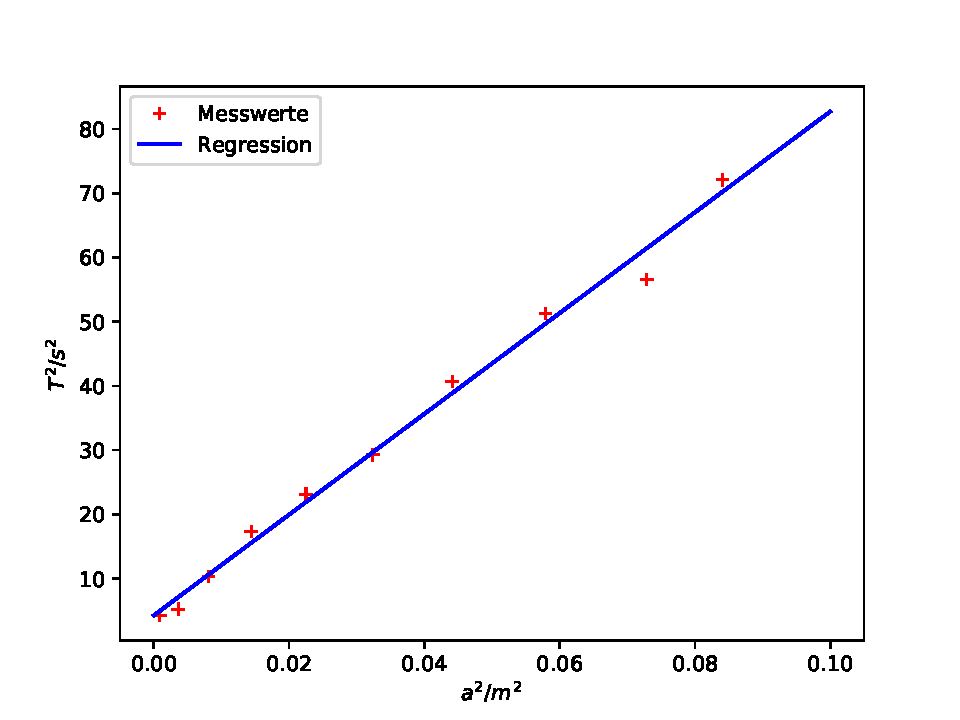
\includegraphics[width=\textwidth]{plot1.pdf}
  \caption{Die Quadrate der Schwingungsdauer gegenüber den Abstandsquadraten}
\end{figure}

Die lineare Regression wird mittels Python durchgeführt. Für die Gerade
\begin{align}
  T^2 &= m * a^2 + n\\
\end{align}
ergeben sich die Steigung $m = (784 \pm 26) \frac{s^2}{m^2}$ und der y-Achsenabschnitt $n = (4.3 \pm 1.1) s^2$.

Für die Berechnung des Eigenträgheitsmoments der Drillachse wird Formel () und die Formel
\begin{align}
I_{Stange} &= \frac{1}{12} \cdot m_{Stange} \cdot H_{Stange}^2
\end{align}
für einen langgen dünnen Stab verwendet. Mithilfe von
\begin{align}
  I_D        &= I_{ges} - 2 \cdot I_{Z} - I_{Stange}\\
             &= \frac{b \cdot D_{dyn}}{4 \pi^2} - 2 \cdot I_{Z} - I_{Stange}\\
\end{align}
lässt sich das Eigenträgheitsmoment von
\begin{equation}
  I_D = (-2.83 \pm 0.000)\cdot10^{-3} \symup{kg m^2}
\end{equation}

%Trägheitsmoment Zylinder
Zu Beginn der Messung werden von dem ausgewählten Zylinder die Radius, Höhe und Masse gemessen:
\begin{align}
  r_Z &= 0.04  \symup{m} \\
  h_Z &= 0.14  \symup{m} \\
  m_Z &= 0.8995  \symup{kg}
\end{align}
Anhand der Werte wird das theoretische Trägheitsmoment bestimmt:
begin{equation}
  I_{Zylinder,theo} = \frac{1}{2} m_Z \cdot r_Z^2 = 0.000720 \,\, \symup{kg m^2}
\end{equation}

\begin{table}
  \centering
  \caption{Schwingungsdauer eines Zylinders}
  \begin{tabular}{c c}
    \toprule
    $\text{Messung}$ & $\text{Dauer\, \, in \, \,s}$
    \midrule
     1 & 1.41\\
     2 & 1.35\\
     3 & 1.32\\
     4 & 1.41\\
     5 & 1.40\\
    \bottomrule
  \end{tabular}
\end{table}
Für die Schwingungsdauer ergibt sich dadurch
\begin{equation}
  T_{Zylinder} = (1.378 \pm 0.018) \symup{s}.
\end{equation}
und für das Trägheitsmoment des Zylinder
\begin{equation}
  I_{Zylinder,exp} = (0.0000198 \pm 0.000000)  \symup{kg m^2} %Fehler und Wert komisch, D=?
\end{equation}
